\documentclass[a4paper,12pt]{report}
\usepackage{color}
\usepackage{hyperref}
\hypersetup{
    colorlinks,
    citecolor=black,
    filecolor=black,
    linkcolor=black,
    urlcolor=black
}
\setcounter{secnumdepth}{0}
\usepackage{graphicx}
\usepackage{epstopdf}
\epstopdfsetup{outdir=./}
\usepackage{amsmath}
\usepackage[table,xcdraw]{xcolor}
\usepackage{amssymb}
\usepackage{listings}
\definecolor{anti-flashwhite}{rgb}{0.95, 0.95, 0.96}
\lstset{
	language=C++,
    basicstyle=\ttfamily,
    keywordstyle=\color{blue}\ttfamily,
    stringstyle=\color{red}\ttfamily,
	commentstyle=\color{green}\ttfamily,
    morecomment=[l][\color{magenta}]{\#},
    backgroundcolor=\color{anti-flashwhite}
}
\begin{document}
\title{
\textbf{Operating Systems - II: CS3523}\\~\\
\begin{large}
\textbf{Lab Exam}\\
\end{large}
\begin{large}
\textbf{Report}
\end{large}
}
\author{\textbf{Sagar Jain - CS17BTECH11034}\\}
\maketitle
\begin{large}
\tableofcontents
\end{large}
\newpage
\section{Program Design}
I have extended the mutual exclusion problem to the class mutual exclusion problem in the following way:
\begin{enumerate}
\item I  have used additional semaphore locks to make sure that only one class of threads can be in the critical section at any one point of time.
\item I have used a special bool array to make sure that not more than one threads belonging to the same class are waiting for the class semaphore. The other threads belonging to the same class wait for  the class to change to their respetive class while the thread waiting on the class semaohore will set the class to its class once it is into the critical section.
\item I keep track of the number of threads of the current class that are in the critical sectin, when this number hits 0, I signal to the class semaphore.
\end{enumerate}
\subsection{Conversion to Normal Mutual Exclusion}
The following changes were made to convert the algorithm.
\begin{enumerate}
\item Change number of classes to number of threads.
\item Change bool array length to number of threads.
\item This essentially maps every thread to a class and thus every class(thread) is run mutually exclusively.
\end{enumerate}
\section{Program Output}
The program outputs a file. The log file contains discrete events of the threads entering and exiting the critical section\\\\
\textbf{Example Output}:\\\\
\textbf{Log File}:\\\\
\textit{0 th CS entry at 17:47:41 by thread 4 for session 4.\\
0 th CS exit at 17:47:41 by thread 4 for session 4.\\
1 th CS request at 17:47:42 by thread 4 for session 4.\\
1 th CS entry at 17:47:42 by thread 4 for session 4.\\
0 th CS entry at 17:47:41 by thread 0 for session 4.\\
0 th CS request at 17:47:41 by thread 9 for session 3.\\
0 th CS request at 17:47:41 by thread 8 for session 5.\\
1 th CS exit at 17:47:42 by thread 4 for session 4.\\
2 th CS request at 17:47:42 by thread 4 for session 2.\\
0 th CS request at 17:47:42 by thread 15 for session 1.\\
0 th CS exit at 17:47:42 by thread 0 for session 4.\\
0 th CS entry at 17:47:42 by thread 2 for session 2.\\\\}

\newpage
\section{Results \& Graphs}
\begin{center}
\begin{large}
\textbf{Average Waiting Times For Class Mutual Exclusion and Simple Mutual Exclusion with Increasing Number of Threads}\\
\end{large}
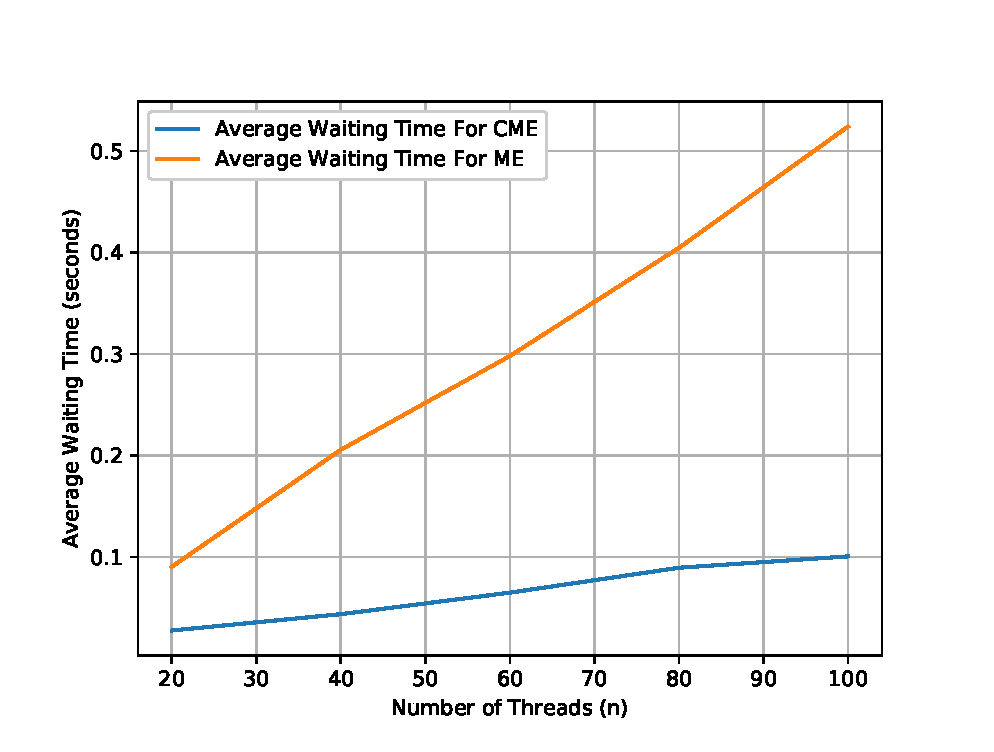
\includegraphics[scale=1]{./graphClass.eps}
\end{center}
\newpage
\section{Explaination of Results}
\begin{enumerate}
\item The time taken by the simple mutual exclusion is constanty more than the time taken by the Class Mutual Exclusion.
\item This is explained by the fact that at any moment of time the number of threads executing in the class mutual exclusion is $\geq1$ while in simple mutual exclusion the number of threads is $=1$.
\item Clearly the throughput for CME is higher than Simple Mutual Exclusion.
\item The rate of increase of Average time is also higher for the Simple Mutual Exclusion since along with number of threads increasing the number of threads fighting for every semaphore is also increasing.
\end{enumerate}
\end{document}